\section{Implementation}
\label{sec:implementation}

To test whether it is possible to prioritize PRs we have designed a service that automatically tries to do just that.

Our implementation of the service consists of several components.
Figure~\ref{fig:architecture} shows a global overview of the architecture.
The \prioritizer service uses two main data sources: GitHub and the \ghtorrent project.
The latter provides a message queue which can be used to subscribe to pull request events.
When such an event arrives the \emph{watcher} component of the \prioritizer is notified (1) and starts prioritizing the project (2).
When the \emph{analyzer} gets a prioritization request it fetches the list of PRs from GitHub (3).
At the same time it fetches the pull request contents to the local Git clone.
When the data is fetched the analyzer starts enriching the PR list with data from the local clone and \ghtorrent (4).
This step calculates and adds several of the features to the PRs.
The data is now ready to be processed by the \emph{predictor} (5) which gives a certain rank to the PRs.
After the ordered list is returned to the analyzer (6), the output is generated and available for the \emph{visualizer} (7).
Details about the different components are discussed in the following sections.

\begin{figure}
  \centering
  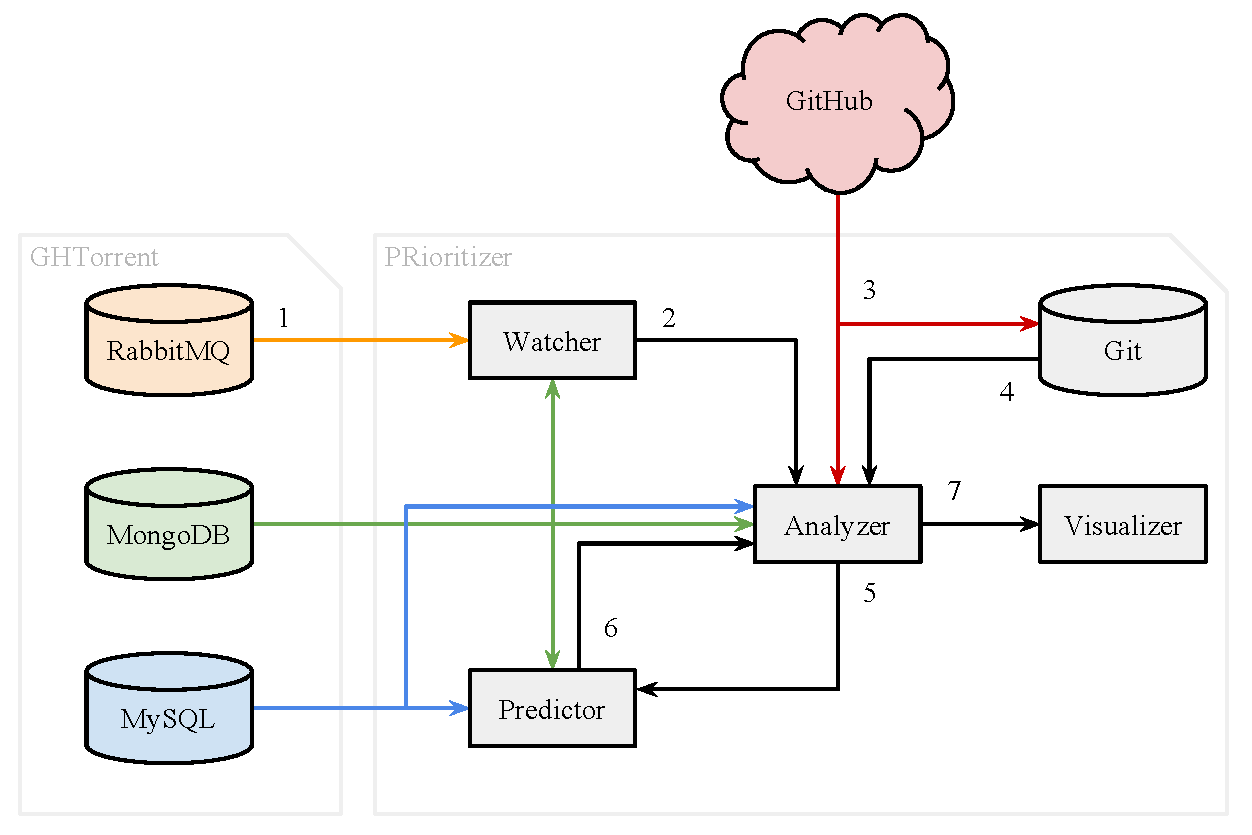
\includegraphics[width=0.5\textwidth]{../figs/architecture.pdf}
  \caption[Diagram of the architecture]
   {Diagram of the architecture. It shows the different data sources and components used by the \prioritizer service.}
  \label{fig:architecture}
\end{figure}

\begin{description}
\item[Watcher]
At the beginning of the chain we have the watcher, it is implemented in the Scala programming language.
The watcher continuously listens to pull request event from \ghtorrent via a RabbitMQ message queue.
Pull request events are triggered when a PR is assigned, unassigned, labeled, unlabeled, opened, closed, reopened, or synchronized.
The PR events of all public repositories on GitHub are received by the watcher.
Incoming events from repositories that are not currently tracked are discarded by the watcher.
If an event is received from a tracked repository the analyzer is invoked for that specific repository.

\item[Analyzer]
The component at the center of the service is the analyzer, it is also implemented in Scala.
When the analyzer kicks in, it receives a repository name from the watcher.
An up-to-date list of open PRs for that repository is fetched from GitHub through the GitHub \api.
In parallel the local git clone is updated with commits of the latest PRs.
At the time both processes are finished, the list with PRs is enriched with data from \ghtorrent as well as the local git clone.

The enrichment process adds e.g. information about the pull request author like the \emph{accept rate}, the \emph{contributor rate} and others described in section~\ref{sec:features}.
To retrieve information like the mergability and the \emph{pairwise conflicts} of the PRs the local git clone is used.
Because of the $O(n^2)$ nature of the pairwise conflict process, this is the most time consuming feature of the service.
After the enrichment process is done, the list is written to a repository specific cache.
This enables a faster enriching process in future runs, especially the pairwise conflict check benefits from the cache.

Some of the enrichment information (e.g. the mergability or number of comments) is also available directly via the GitHub \api.
However, this data is only present when requesting a single PR, whereas a request for a list of 100 PRs lacks this sort of data.
This means that if we want this data directly from GitHub we have to create one \api request per pull request.
When prioritizing PRs for a large amount of repositories it consumes also a large amount of \api requests and reaches GitHub's maximum of 5,000 requests/hour quickly.
So, our solution to this problem is to use \ghtorrent instead.

Before the final output is written to the disk, the predictor is invoked on the enriched PR list.
A list of ordered PRs is returned back from the predictor to the analyzer.
Details about this process are in the next paragraph.
The analyzer completes its process with writing the ordered list of PRs to the disk in JSON format, which will be picked up by the visualizer.

\item[Predictor]
The predictor assigns a rank to every pull request, it is partly written in Scala and partly in R.
When the predictor receiver a list of PRs it first checks if there is already a up-to-date prediction model.
If this is not the case, the first step is to train the prediction model on a set of PRs from the past.

The training process consists of two phases, first the historical data must be retrieved and secondly the actual model must be trained.
Information about closed pull request, their comments and their authors is harvested from \ghtorrent.
Once all data is fetched, the lifetime of each PR is divided into time windows to construct the training data as explained in section~\ref{sec:training}.
When the training set is complete it is passed to the R program which trains the prediction model.

The Random Forest machine learning algorithm, called in R, learns what features are important for dividing the PRs in two classifications (important vs. not important).
The resulting model is saved to the disk for later use when predicting the ranks.

Once we have a up-to-date prediction model, we can use it for ordering the PR list.
The list and the model are feeded to the prediction algorithm in R.
Using the prediction model each PR is given a probability that it belongs to the \emph{important} cluster.
A PR with a high probability means that it is more likely to receive an event or action (from the user) soon.
We interpret PRs with a high probability as PRs that need attention, therefore the ranked list of PRs is obtained by ordering the list on the importance probability from high to low.
The final list is then returned to the analyzer.

\item[Visualizer]
The visualizer is a user interface for the ordered list, it is a web application written in HTML and Javascript.
An example view of the interface can be seen in figure~\ref{fig:ui}.
To make the development faster and easier we used AngularJS, a Javascript framework.
The visualizer is a static website which accesses the JSON produced by the analyzer.
When a specific repository is requested by the user, the corresponsding JSON file is parsed and showed on the web page.

The list is automatically sorted on the rank outputted by the predictor.
However, the user is also able to sort or filter manually on different fields and features.
On GitHub has only a limited set of fields available to sort and filter on.
The visualizer interface provides more sort and filter options based on the features from section~\ref{sec:features} e.g. conflicts, author properties or size.
Sorting on something trivial as the size of a PR is not support on GitHub while many integrators use it as manual prioritization feature \cite{GZSD15}.

The interface tells users on which PR they have to focus first.
However, to actually take action the user still has to go to GitHub's interface.
To make it easier for the user each PR in the list has a link to the GitHub version.
Futhermore, if a user wants more information about a specific PR, he/she can click the PR to reveal more details about the features.
\end{description}

\begin{figure}
  \centering
  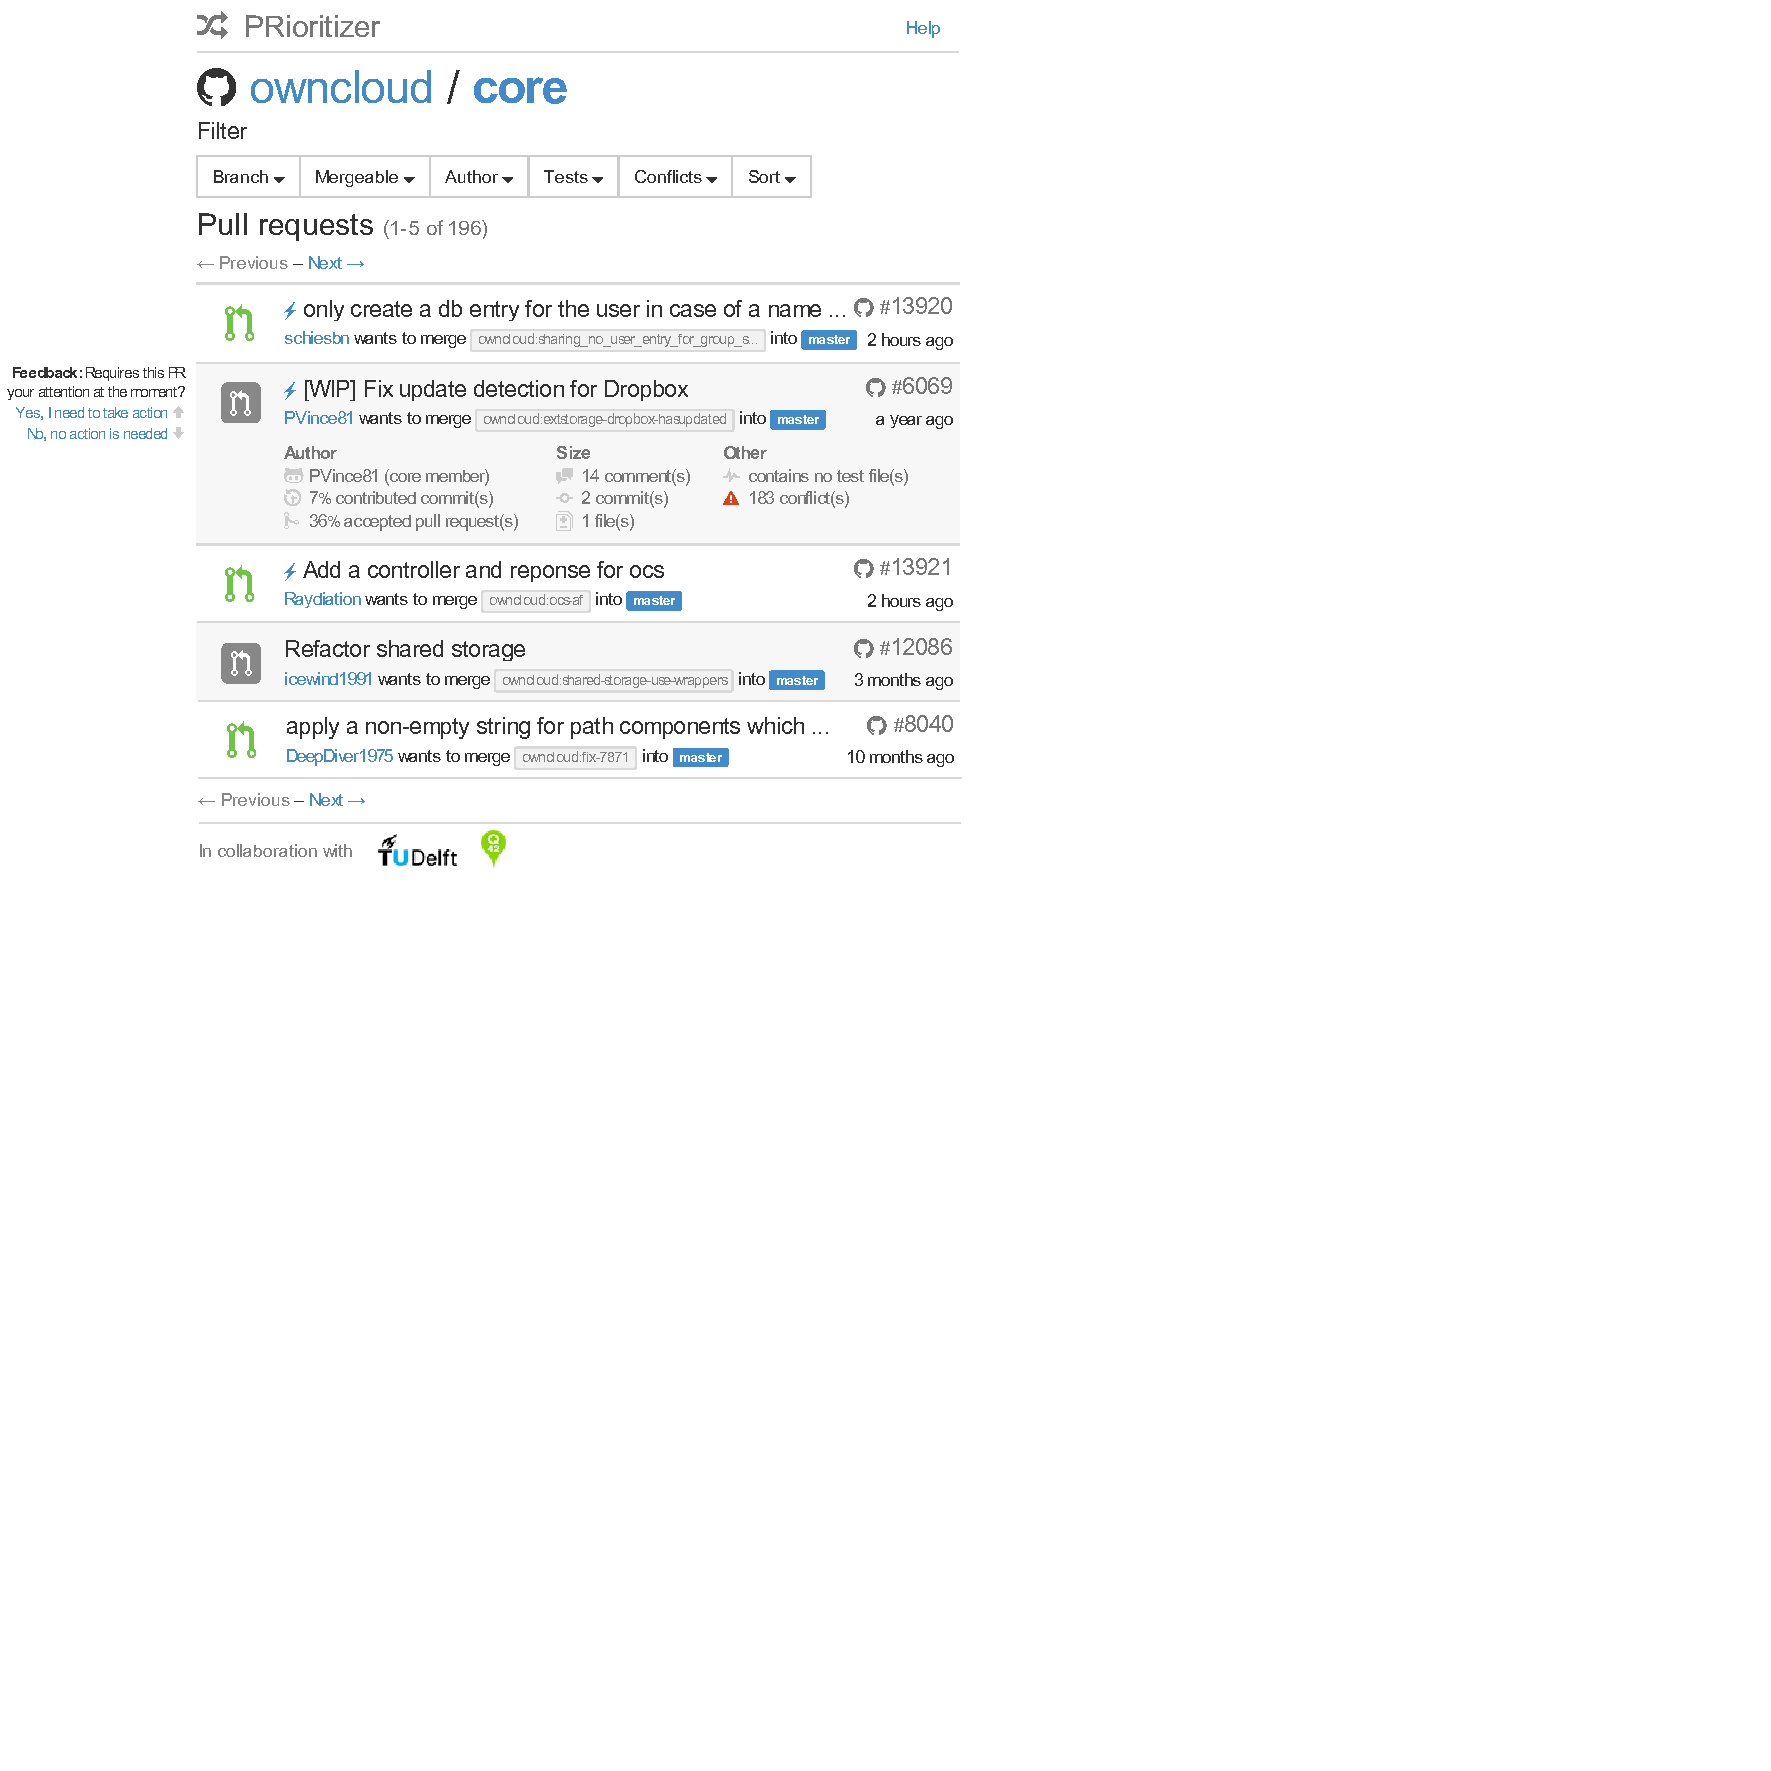
\includegraphics[width=0.5\textwidth]{../figs/interface.pdf}
  \caption[The user interface]
   {The user interface. It shows an ordered list of pull requests that need attention.}
  \label{fig:ui}
\end{figure}
